\begin{figure}
    \centering
    \setlength{\belowcaptionskip}{10pt}
    \caption{Architecture of Algorithm}
    \label{ac-figure}
    \tikzstyle{rec} = [rectangle, rounded corners=2mm, fill = yellow!50, minimum width = 2cm, minimum height = 1cm, text centered, draw = black, align=center]
    \tikzstyle{rec1} = [rectangle, rounded corners=2mm, fill = red!50, minimum width = 2cm, minimum height = 1cm, text centered, draw = black, align=center]
    \tikzstyle{rec2} = [rectangle, rounded corners=2mm, fill = blue!50, minimum width = 2cm, minimum height = 1cm, text centered, draw = black, align=center]
    \tikzstyle{arrow} = [thick, ->, draw = blue]
    \tikzstyle{arrow1} = [thick, ->, draw = red]
    \tikzstyle{line} = [thick, -, draw = blue]
    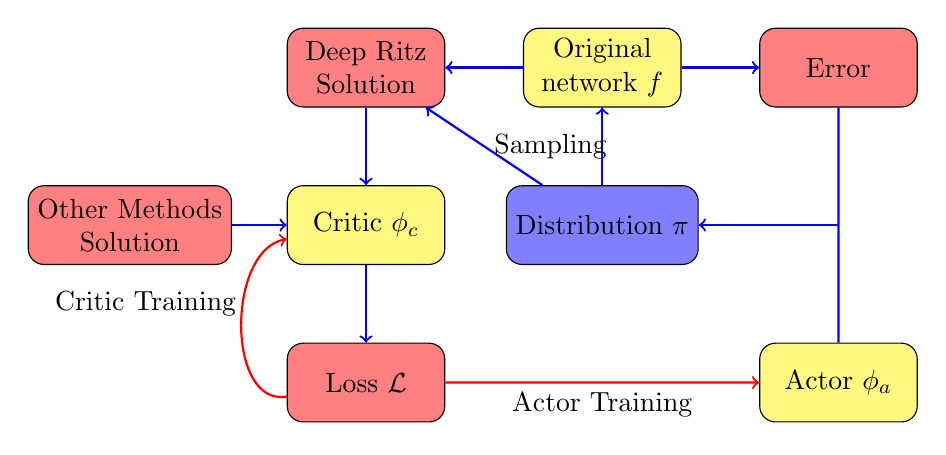
\begin{tikzpicture}[node distance = 1cm]
    	\node(origin)[rec]{Original\\network $f$};
        \node(error)[rec1, right of = origin, xshift = 2cm]{Error};
        \node(actor)[rec, below of = error, yshift = -3cm]{Actor $\phi_{a}$};
		\node(distribution)[rec2, below of = origin, yshift = -1cm]{Distribution $\pi$};
		\node(deep_ritz)[rec1, left of = origin, xshift = -2cm]{Deep Ritz\\Solution};
		\node(critic)[rec, below of = deep_ritz, yshift = -1cm]{Critic $\phi_{c}$};
		\node(others)[rec1, left of = critic, xshift = -2cm]{Other Methods\\Solution};
		\node(critic_loss)[rec1, below of = critic, yshift = -1cm]{Loss $\mathcal{L}$};
		\node(train_critic) at (-5.8, -3) {Critic Training};
        \draw[arrow] (origin) -- (error);
        \draw[arrow] (distribution) -- (origin);
        \draw[arrow] (distribution) -- (deep_ritz) node[midway, right] {Sampling};
        \draw[line] (error) -- (3, -2);
        \draw[line] (actor) -- (3, -2);
        \draw[arrow] (3, -2) -- (distribution);
        \draw[arrow] (origin) -- (deep_ritz);
        \draw[arrow] (deep_ritz) -- (critic);
        \draw[arrow] (others) -- (critic);
        \draw[arrow] (critic) -- (critic_loss);
        \draw[arrow1] (critic_loss) to [out=190, in=190] (critic);
        \draw[arrow1] (critic_loss) -- (actor) node[midway, below] {Actor Training};
    \end{tikzpicture}
\end{figure}